\section{Results}

All results describing the correctness of the simulation or discussing the closeness of the simulation to an analytical
result are done using the single-threaded mode. This is because this makes the result of the simulation deterministic,
and so it does not matter which machine the test was run on. For results that measure performance, the machine and options
for the simulation used will be specified. There are times when the number of threads affected the correctness of the
result.

\subsection{The $\sin(x)$ Potential}

	\begin{figure}[h]
	\centering
	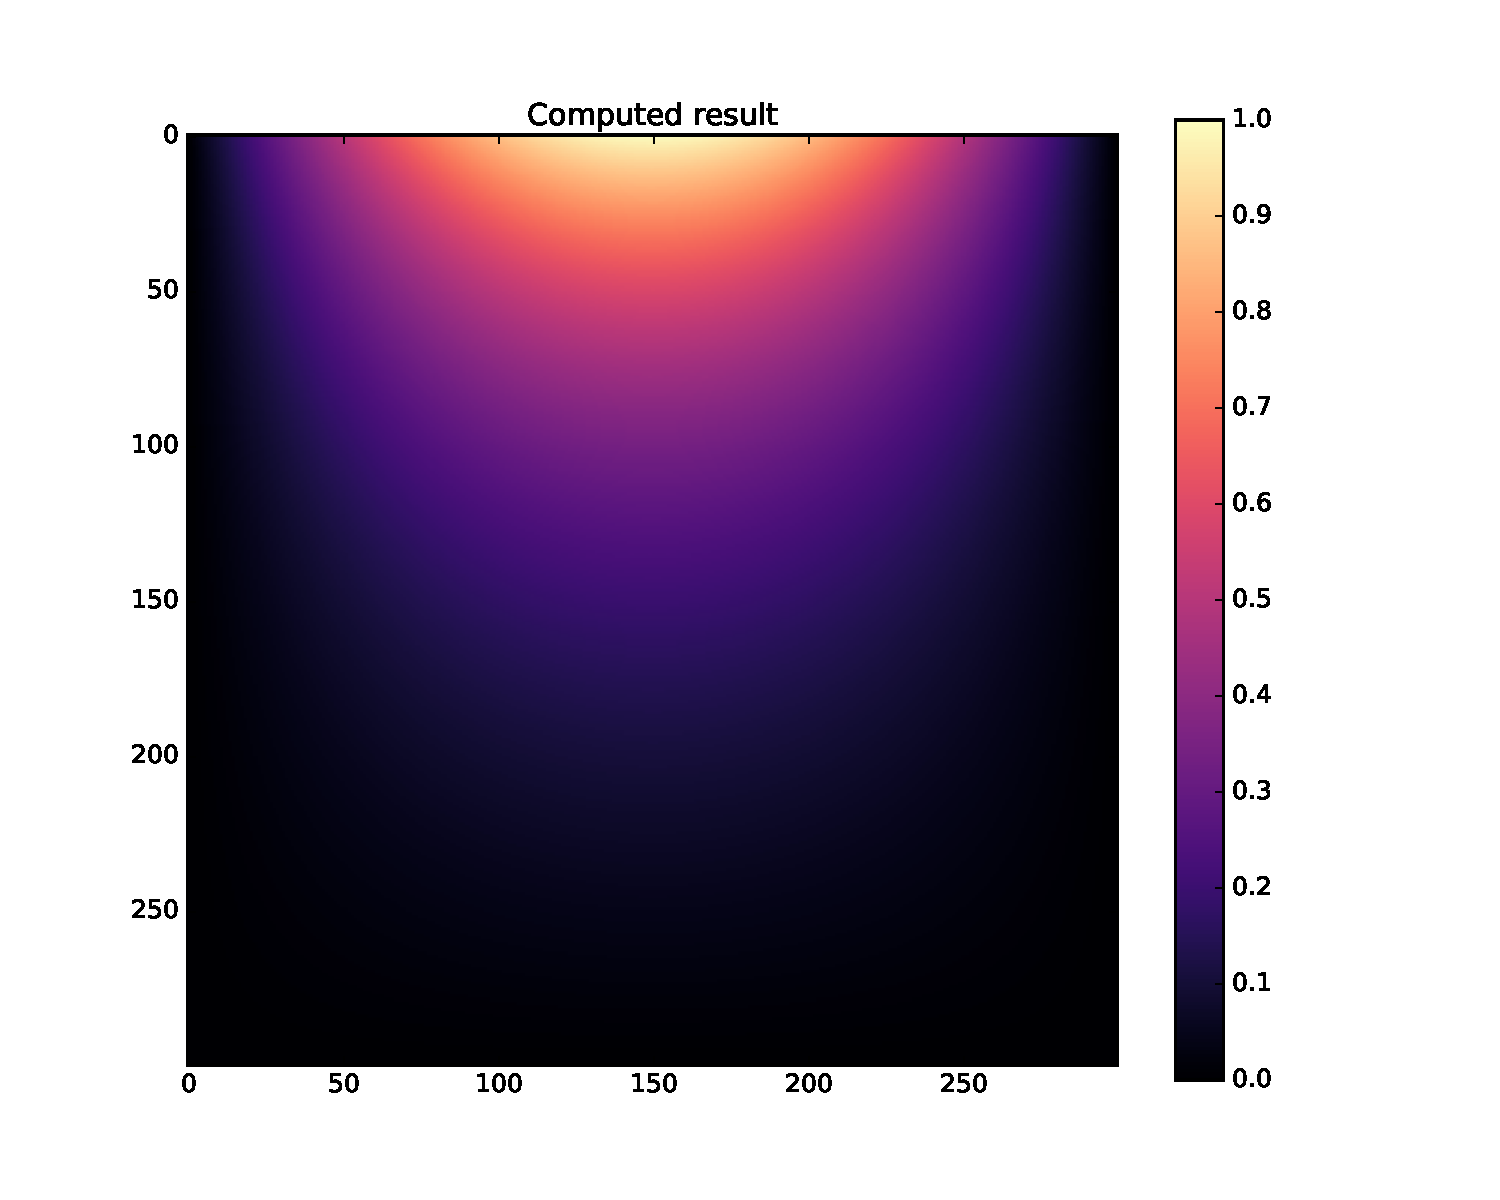
\includegraphics[width=1.1\linewidth]{sin300_calc.pdf}
	\caption{Simplistic view of CPU and RAM.} 
	\label{fig:sin-result}
	\end{figure}

	\begin{figure}[h]
	\centering
	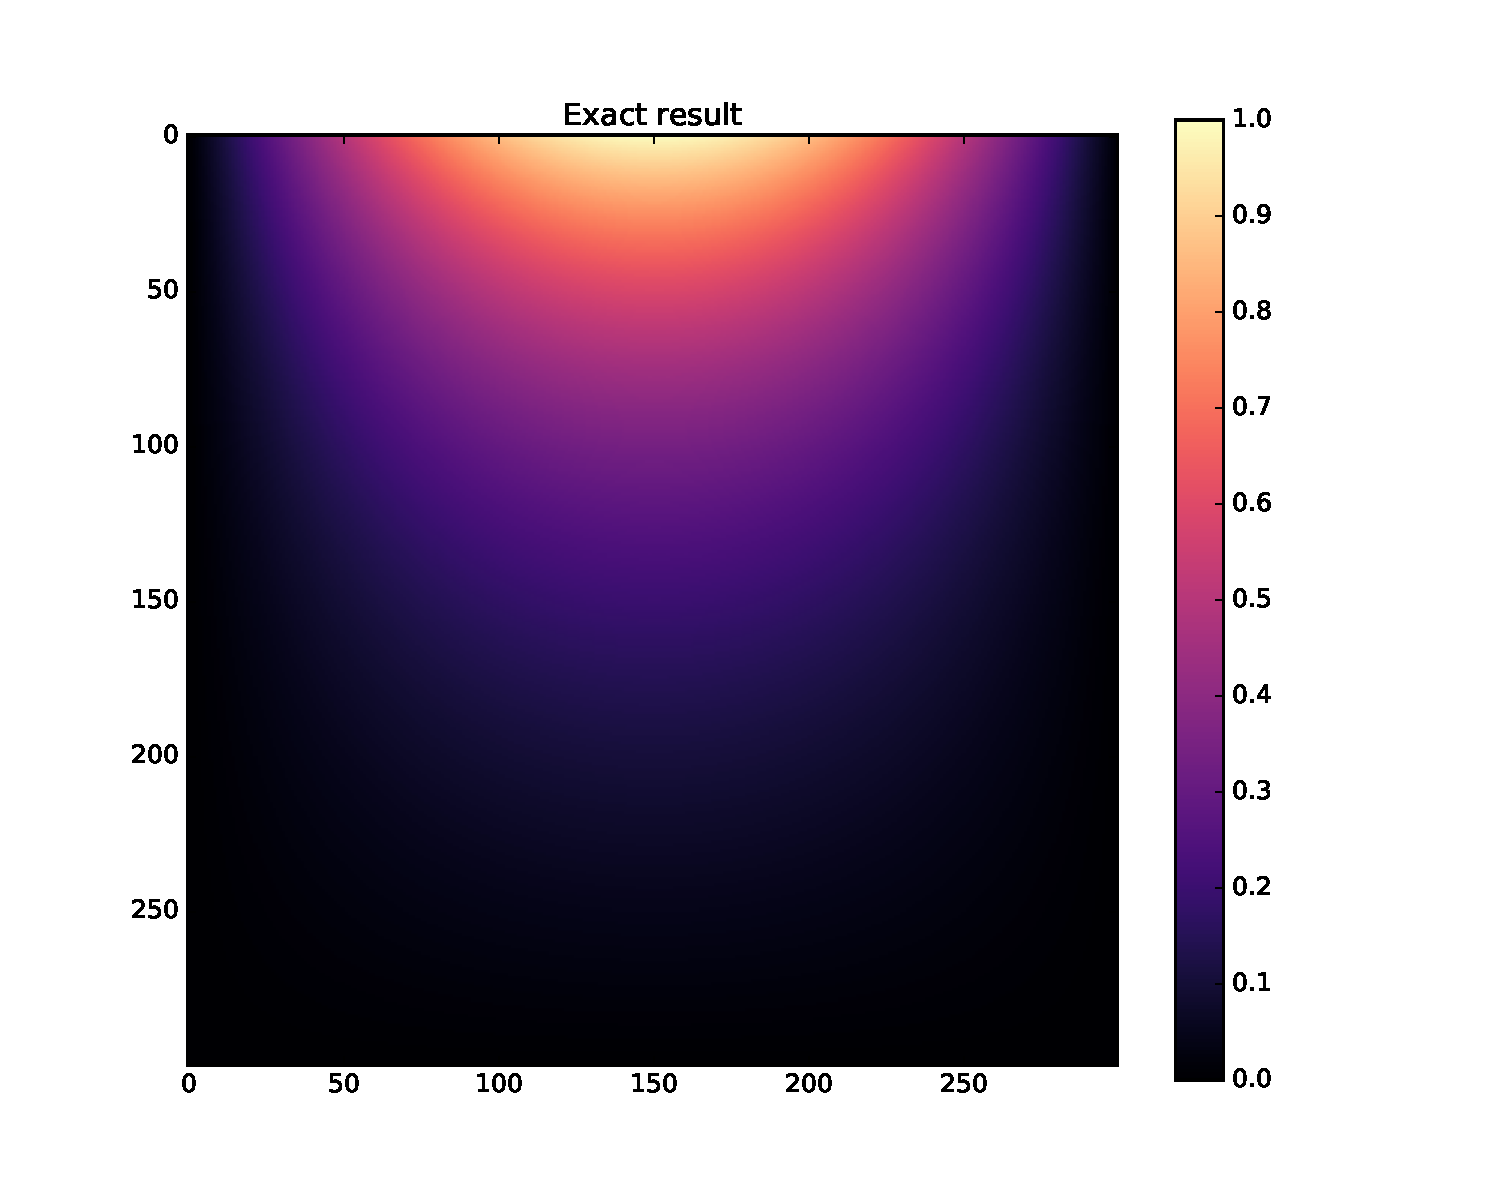
\includegraphics[width=1.1\linewidth]{sin300_exact.pdf}
	\caption{More realistic view of CPU and RAM.}
	\label{fig:sin-analytic}
	\end{figure}

Figure~\ref{fig:sin-result} shows the output of the solver program in single-threaded mode when given the $\sin(x)$ along one side
potential, plotted with the Python library matplotlib. The configuration has a grid size of 300 by 300. It matches very well with the analytical result, which
is
$$\frac{\sinh(y \pi / n)}{\sinh(\pi)} \sin(x \pi / n),$$
and is shown plotted in a similar way in figure~\ref{fig:sin-analytic}. The difference between the calculated result and the
analytical result is shown in figure~\ref{fig:sin-difference}. The values shown in the difference map are small compared
to the values in the result in all locations except the corners at the top, where the simulation does diverge somewhat, 
but never reaches values which are hugely divergence from the analytical result. Using the root-mean-square error statistic
described earlier, we have calculated that the RMS error in this simulation to be SOME NUMBER.


	\begin{figure}[h]
	\centering
	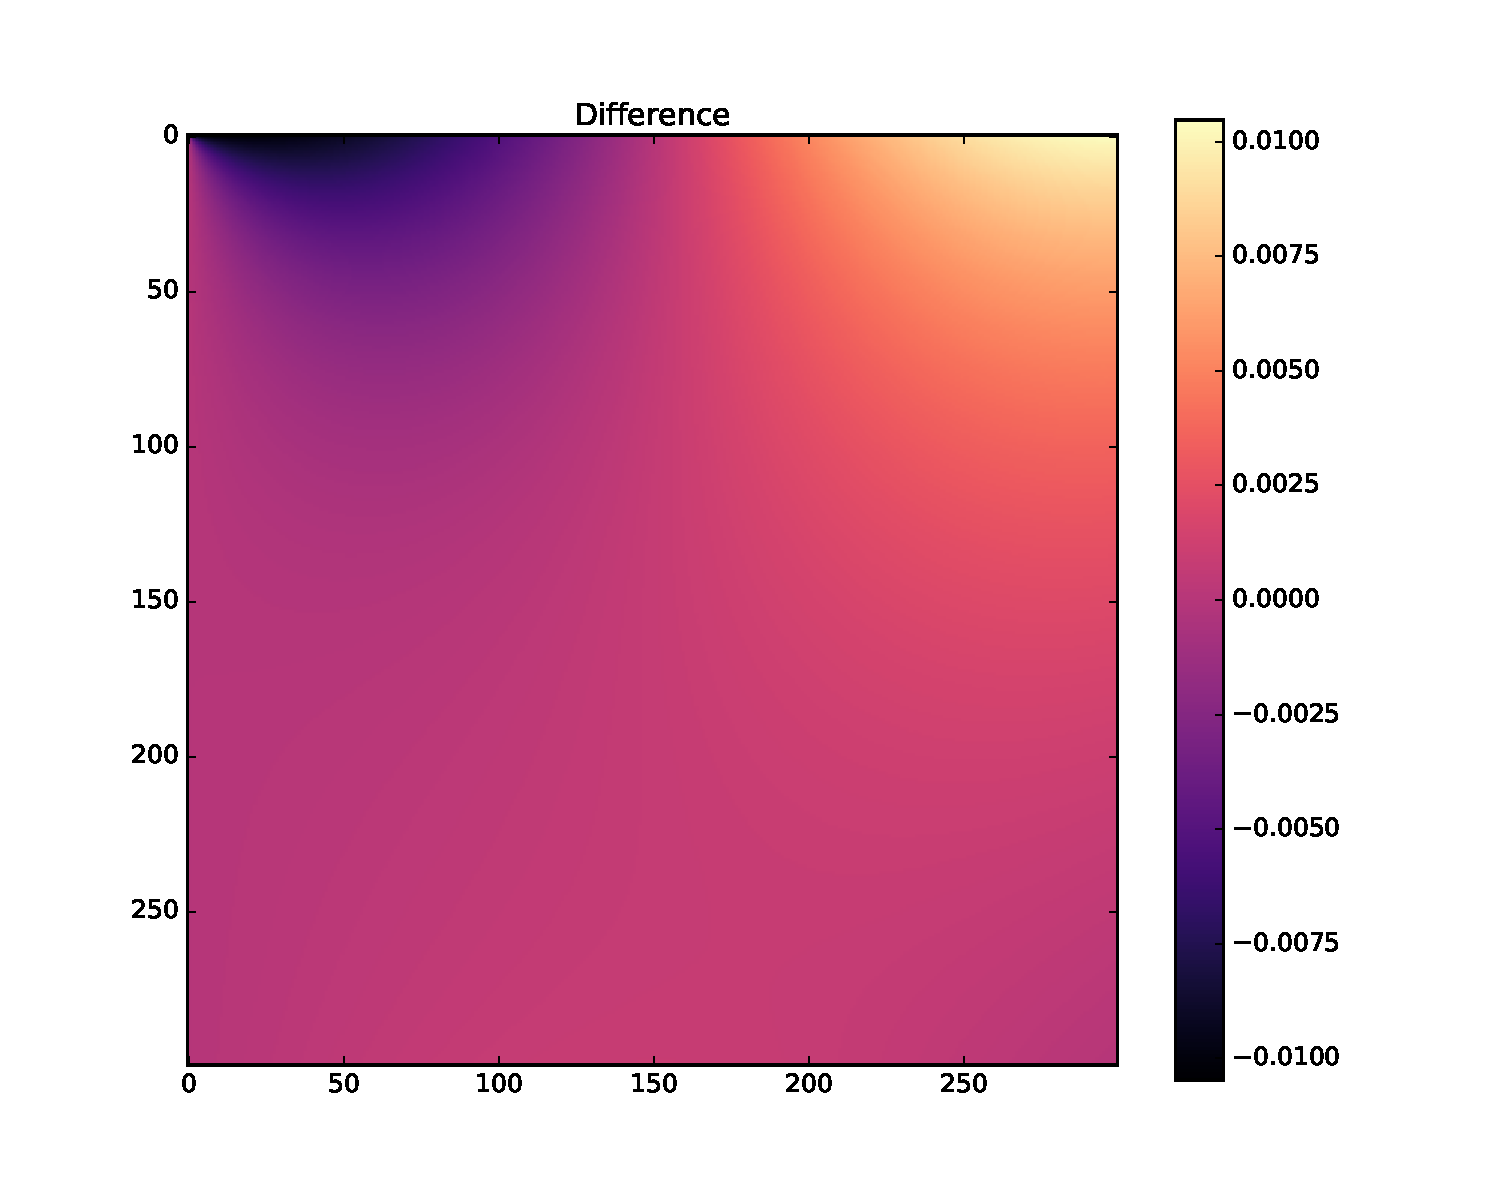
\includegraphics[width=1.1\linewidth]{sin300_diff.pdf}
	\caption{More realistic view of CPU and RAM.}
	\label{fig:sin-difference}
	\end{figure}

\subsection{Fitting to a $1/r^2$ Dipole Potential}

The dipole configuration had a grid size of 400 by 400, with all walls given a Dirichlet boundary condition
of zero. Two charges were placed near the center 10 cells apart with an arbitrary but equal and opposite charge.
The result of this simulation is shown in figure~\ref{fig:dipole-cont}, with the addition of constant-potential
contour lines. The simulation shows two opposite charges which near perfectly mirror each other. The vertical
line in the center represents a constant potential contour with a value of zero, which is expected from an
electric dipole. This is another excellent verifier that the simulation is producing correct results.

\begin{figure}[h]
	\centering
	\center
	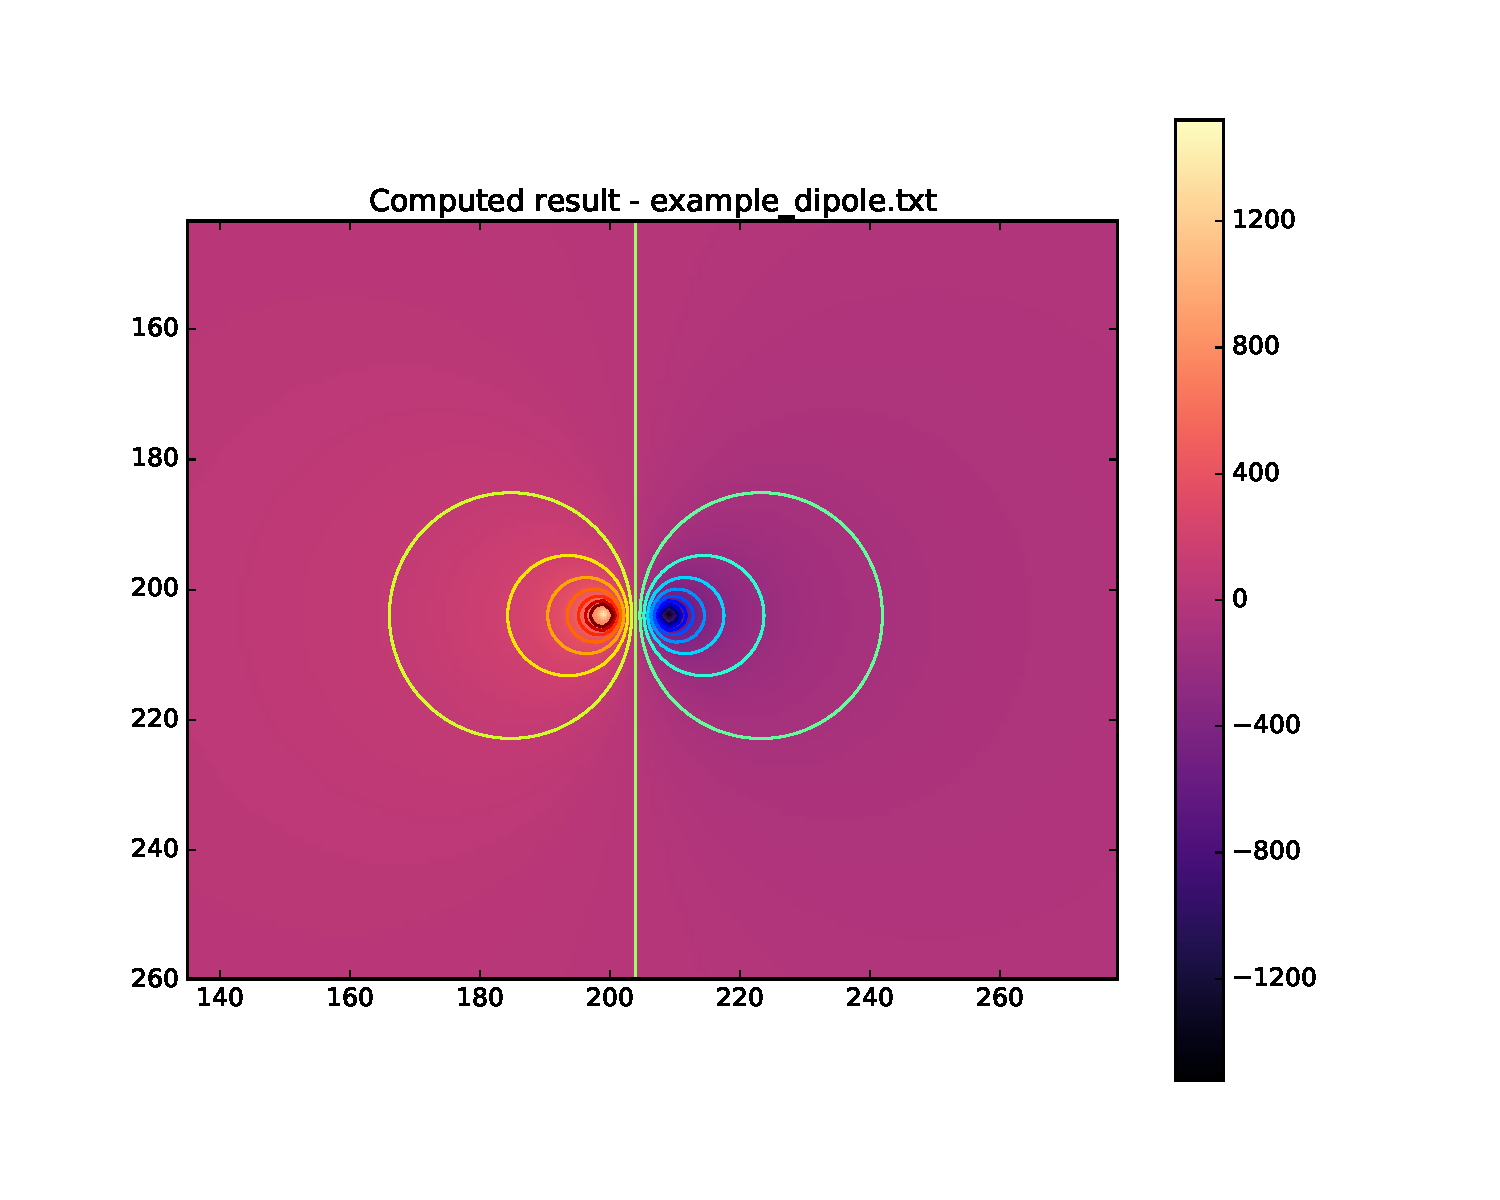
\includegraphics[width=1.1\linewidth]{dipole_contours.pdf}
	\caption{Fitting a $1/r^2$ curve to the calculated dipole potential.} \label{fig:dipole-cont}
	\end{figure}

The potential was then measured at locations increasing in distance from the dipole in an arbitrary direction.
These data were then plotted using gnuplot, and a line of the form $y(x) = A + B / (r-r_0)^2$ was fit to the
data, which is shown in figure~\ref{fig:dipole-fit} The fit is excellent, confirming that the program had properly simulated an electric dipole. The error
bars on the data points come from the difference between successive iterations at the end of the simulation of
the dipole. They are very small, but non-zero.



	\begin{figure}[h]
	\centering
	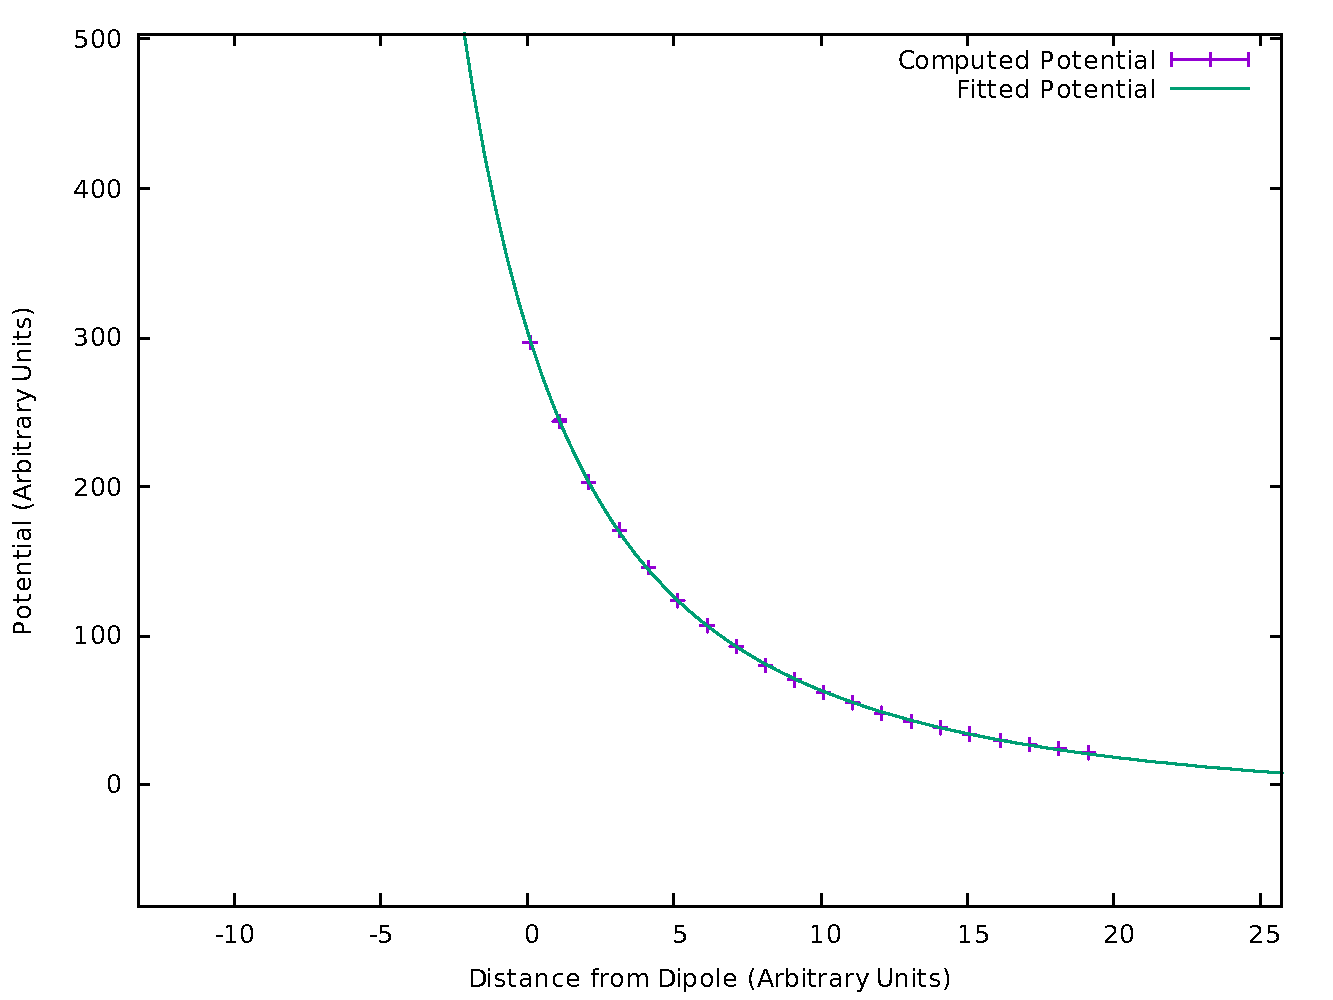
\includegraphics[width=\linewidth]{dipole_fit.pdf}
	\caption{Fitting a $1/r^2$ curve to the calculated dipole potential.} \label{fig:dipole-fit}
	\end{figure}

The dipole is an example which lends itself to presenting another feature of the solver program. If passed the
$\texttt{-V}$ option, it will take the negative gradient of the result and plot that as a vector field. This has
the effect of plotting the electric field of the result of the simulation, which for the dipole is shown in
figure~\ref{fig:dipole-field}.

	\begin{figure}[h]
	\centering
	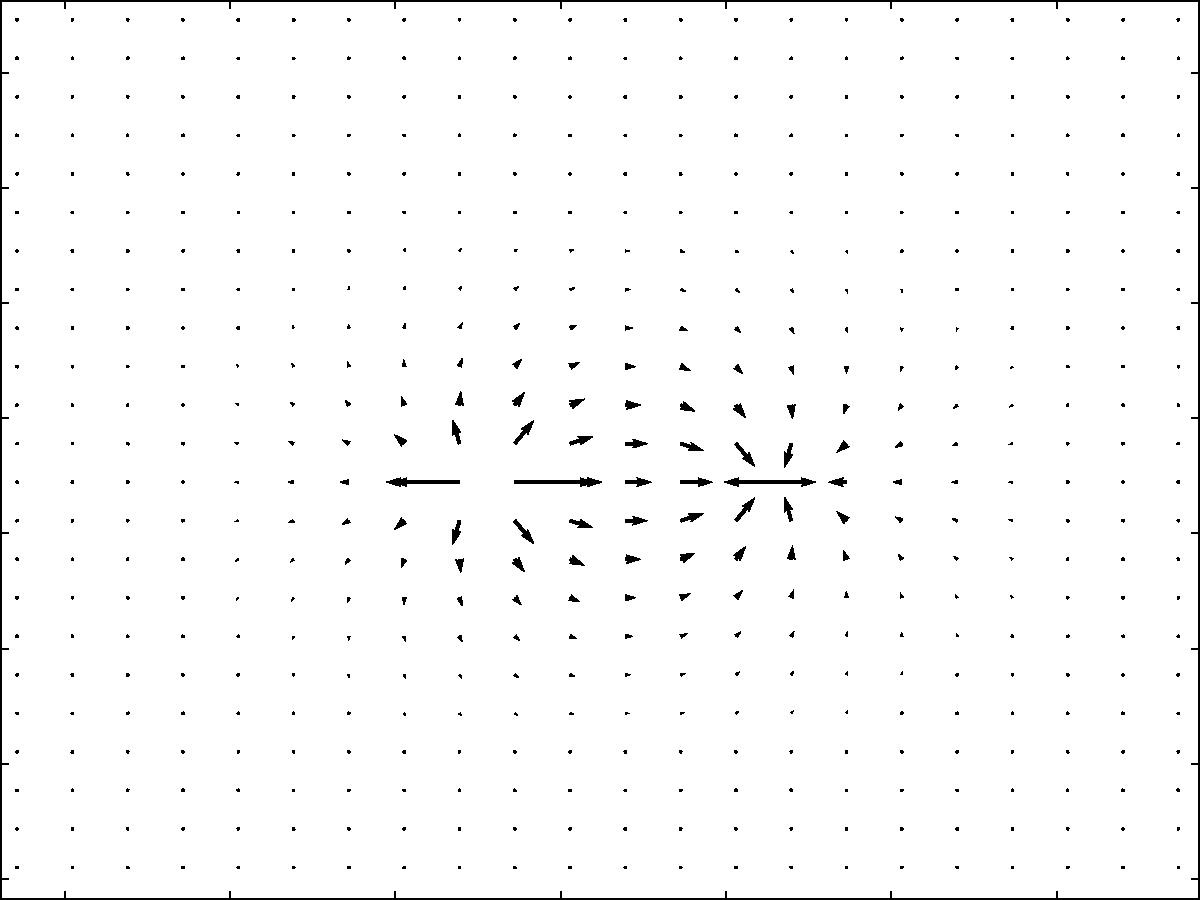
\includegraphics[width=0.7\linewidth]{dipole_field.pdf}
	\caption{Fitting a $1/r^2$ curve to the calculated dipole potential.} \label{fig:dipole-field}
	\end{figure}


\subsection{Performance}


Figure~\ref{fig:perf-sizes} shows the performance in iterations per second for a varying grid size for given
configuration, in this case the $\sin(x)$ along a wall potential. The performance tests were run square grids
of size 50 by 50, 300 by 300, and 1000 by 1000. For each grid size, 4 different simulation options were given:
single-threaded non-SIMD, single-threaded SIMD, multi-threaded with 4 threads non-SIMD, and multi-threaded
with 4 threads and SIMD.

In the case of the 50 by 50 grid, the performance was similar for all cases
except for multi-threaded with SIMD. I believe the reason that the SIMD multi-threaded version was slower was
due to the manual SIMD code being less cache-friendly, resulting in the threaded versions having more contention.
Both the 300 by 300 case and 1000 by 1000 case display similar performance behavior: the SIMD case is faster than
the non-SIMD case when single threaded, and the SIMD case is slower than the non-SIMD case when multi-threaded.
This can be explained in the same was as it was for the 50 by 50 case. Another characteristic is that the multi-threaded
case (with 4 threads) is faster than the single threaded case. In fact, it is better than I expected it to be.

Additionally, the performance depends heavily on the grid size. This makes sense, as the amount of work needed to be
done per iteration is proportional to the number of cells in the grid, and the number of cells in the grid is $n^2$.
Another note is that the variance on the performance is significantly higher for all of the multi-threaded cases.
This is because having multiple threads increases the program's dependence on the scheduling quirks of the operating
system. Finally, the variance for the 50 by 50 case multi-threaded versions are significantly higher than all other
variances for the other multi-threaded cases. I believe that this is because the overhead of managing threads compared
to how much work they actually have to do is large in this case compared to the other cases.


\begin{figure}[h]
	\centering
	\pgfplotstableread{
		0 55642.1 3747.52    54100.9 3401     53724.2 13306.44    44877.5 9672
		1 1504 30.6    1461 15     3119 269    2333 313
		2 132.845 1.36    127.085 3.45     297.9 23.13    222.8 26.7
	}\dataset
	\begin{tikzpicture}
    \begin{axis}[
    	xticklabels = {
    		sin50,
    	    sin300,
    	    sin1000,
    	},
        xtick=data,
        ymode=log,
            log ticks with fixed point,
        major x tick style = transparent,
        width  = 0.85*\textwidth,
        height = 8cm,
        major x tick style = transparent,
        enlarge x limits=0.25,
        ybar=2*\pgflinewidth,
        bar width=14pt,
        ymajorgrids = true,
        ylabel = {Run time speed (iters/sec)},
        xtick = data,
        major x tick style = {opacity=0},
        minor x tick num = 1,
        minor tick length=2ex,
        ymin=0,
        legend cell align=left,
		legend style={
	        anchor=south east,
	        column sep=1ex
	    },
        ]

\addplot+[error bars/.cd, y dir=both, y explicit] table[x index=0,y index=1, y error index=2] \dataset; %Data1
\addplot+[error bars/.cd, y dir=both, y explicit] table[x index=0,y index=3, y error index=4] \dataset; %Data2
\addplot+[error bars/.cd, y dir=both, y explicit] table[x index=0,y index=5, y error index=6] \dataset; %Data3
\addplot+[error bars/.cd, y dir=both, y explicit] table[x index=0,y index=7, y error index=8] \dataset; %Data3

	\legend{Single Threaded SIMD, Single Threaded, Multithreaded (4 threads), Multithreaded (4 threads) SIMD}
\end{axis}
\end{tikzpicture}
\caption{Different grid sizes for the $\sin(x)$ configuration, and their performance characteristics.}
\label{fig:perf-sizes}
\end{figure}

%		\addplot[ybar,fill=green,mark=none] coordinates {(0,   1513.05)};
% \addplot[ybar,fill=blue,mark=none] coordinates {(0,   1459.24)};
% \addplot[ybar,fill=red] coordinates {(0,   3174.49)};
% \addplot[ybar,fill=orange] coordinates {(0,   2354.03)};

	% \addplot[ybar,fill=green,mark=none] coordinates {(1,   1513.05)};
	% \addplot[ybar,fill=blue,mark=none] coordinates {(1,   1459.24)};
	% \addplot[ybar,fill=red] coordinates {(1,   3174.49)};
	% \addplot[ybar,fill=orange] coordinates {(1,   2354.03)};

	% \addplot[ybar,fill=green,mark=none] coordinates {(2,   1513.05)};
	% \addplot[ybar,fill=blue,mark=none] coordinates {(2,   1459.24)};
	% \addplot[ybar,fill=red] coordinates {(2,   3174.49)};
	% \addplot[ybar,fill=orange] coordinates {(2,   2354.03)};












Figure~\ref{fig:perf-numthreads} shows the performance in iterations per second of the solver when run
with the $\sin(x)$ potential with a grid size of 300 by 300. This was done on computer B, and so was done
only in non-SIMD mode. The results show a significant improvement in performance when using multiple threads
compared to the single threaded case. One may na\"{i}vely have expected the performance to scale linearly
with the number of threads; however, this would be very unlikely. As the number of threads goes up, the amount
of work that can be done in parallel would seem to scale with the number of threads, until one considers processor cache effects (specifically
cache coherency and cache size limitations). This is seen in the case of 4 threads, as it is not 4 times as fast as
the single threaded case, only about 3.2 times as fast. Increasing the number of threads quickly starts giving diminishing
returns, as the 8 threads case is now only slightly better than the 4 threads case. Recall that computer B, on which these
tests are run, has 4 cores with 2 threads each, totally 8 possible threads running in parallel. After the 8 threads case,
we start to see a drop in performance; the 16 and 32 threads case are worse than the 8 threads case. This is because
the machine cannot run more than 8 threads in parallel, so in order to have 16 threads it must rely on the scheduling
of the operating system in order to get work done. In a case of many threads, each doing heave computation and memory accesses
(as is the case here), it does not usually help to increase the number of threads beyond what the machine can handle,
as is shown here.

\begin{figure}[h]
	\centering
	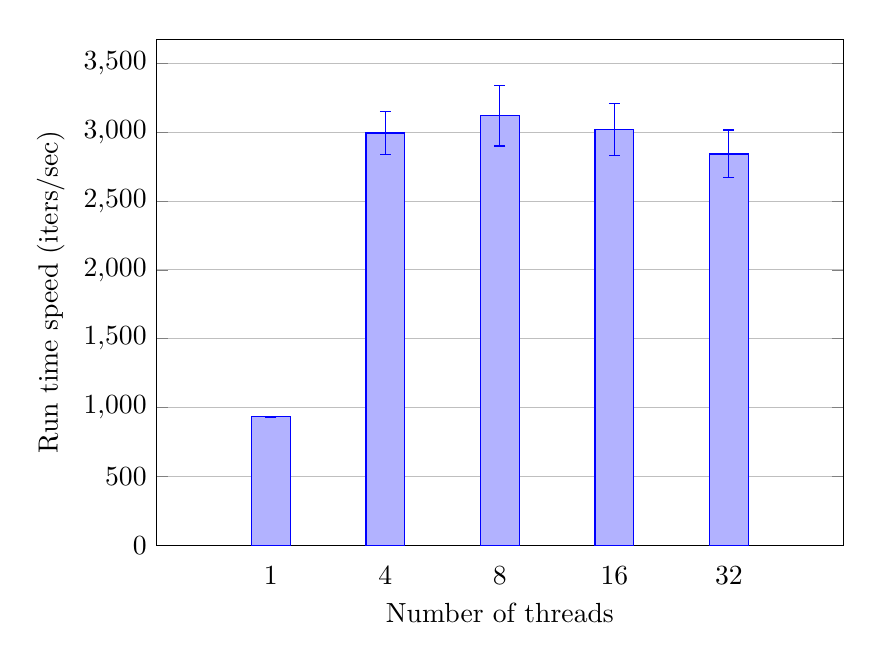
\begin{tikzpicture}
    \begin{axis}[
        xtick=data,
        symbolic x coords={1, 4, 8, 16, 32},
        major x tick style = transparent,
        width  = 0.85*\textwidth,
        height = 8cm,
        major x tick style = transparent,
        ybar=2*\pgflinewidth,
        bar width=14pt,
        ymajorgrids = true,
        ylabel = {Run time speed (iters/sec)},
        xlabel = {Number of threads},
        xtick = data,
        scaled y ticks = false,
        enlarge x limits=0.25,
        ymin=0,
        legend cell align=left,
		legend style={
	        anchor=south east,
	        column sep=1ex
	    },
        ]
            \addplot+[error bars/.cd,
                       y dir=both, y explicit]
                    coordinates {
                    (1, 933.156)  +- (3.612, 3.612)
                    (4, 2994.42)  +- (157.1, 157.1)
                    (8, 3119.1)  +- (219, 219)
                    (16, 3020.6)  +- (190, 190)
                    (32, 2842)  +- (174, 174)
                    };
\end{axis}
\end{tikzpicture}
\caption{Performance results for a varying number of threads in non-SIMD mode. These
tests were done on computer B, using the $\sin(x)$ potential with a grid size of 300 by 300.}
\label{fig:perf-numthreads}
\end{figure}



Furthermore, figure~\ref{fig:err-numthreads} shows that it is disadventagous to run the simulation with
a large number of threads. The RMS error of the simulation compared to the analytical result increases
rapidly with the number of threads. This is also reflected in the result of the simulation, which is
noticably wrong in the case of 16 or higher threads. I believe this to be the result of the way the threads
are synchronized, or more accurately, how they are not. The threads run mostly in isolation, sharing the
grid and doing operations on it without waiting for other threads to complete any of their work. This means
that if one threads runs faster than the others, it may complete a different number of iterations than the other
threads in a given amount of time. This would result in some sections of the grid recieving more iterations
than others, which could have the effect of invalidating the simulation. The alternative method would be
to synchronize the threads, and have them wait for each thread to complete a given iteration before moving on
to the next one. Indeed, this was the original design of the system, and I found it to be so slow compared to
single threaded that I changed the design around to the less accurate but much faster design that is shown here.



\begin{figure}[h]
	\centering
	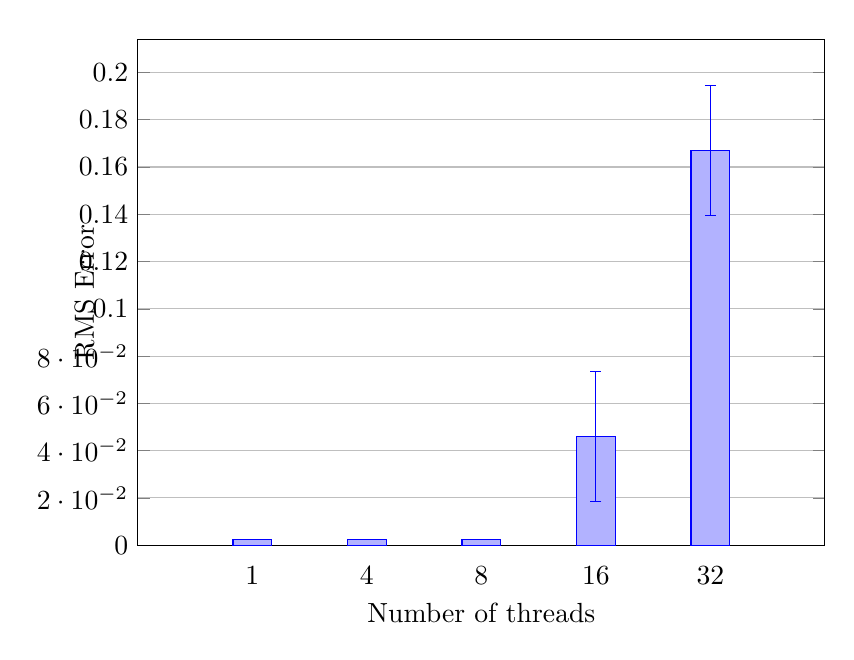
\begin{tikzpicture}
    \begin{axis}[
        xtick=data,
        symbolic x coords={1, 4, 8, 16, 32},
        major x tick style = transparent,
        width  = 0.85*\textwidth,
        height = 8cm,
        major x tick style = transparent,
        ybar=2*\pgflinewidth,
        bar width=14pt,
        ymajorgrids = true,
        ylabel = {RMS Error},
        xlabel = {Number of threads},
        xtick = data,
        y label style={at={(axis description cs:-0.05,.5)},rotate=0,anchor=south},
        enlarge x limits=0.25,
        try min ticks=10,
        ymin=0,
        legend cell align=left,
		legend style={
	        anchor=south east,
	        column sep=1ex
	    },
        ]
            \addplot+[error bars/.cd,
                       y dir=both, y explicit]
                    coordinates {
                    (1, .002544)  +- (0, 0)
                    (4, .002544)  +- (.000000027, .000000027)
                    (8, .002544)  +- (.0000000269, .0000000269)
                    (16, .046)  +- (.0274, .0274)
                    (32, .167)  +- (.0274, .0274)
                    };
\end{axis}
\end{tikzpicture}
\caption{Error results for a varying number of threads in non-SIMD mode. These
tests were done on computer B, using the $\sin(x)$ potential with a grid size of 300 by 300.}
\label{fig:err-numthreads}
\end{figure}



%32 ave: 0.166412 sq: 0.0277446 stddev: 0.00718529
